%----------------------------------------------------------------------------------------
%	PACKAGES AND DOCUMENT CONFIGURATIONS
%----------------------------------------------------------------------------------------
\documentclass[11pt]{article}
\usepackage{amsmath} % Required for some math elements
\usepackage{hyperref} 
\usepackage{xcolor}
\usepackage{lipsum} 
\usepackage{cite}
\usepackage{graphicx} % Required for the inclusion of images
\usepackage{algorithmic}
\usepackage{array}
\usepackage{bookmark}
\usepackage{listings}
\usepackage{amssymb}
\usepackage{enumitem}
\usepackage{pythonhighlight}
\usepackage[T1]{fontenc}
\usepackage{inconsolata}
\usepackage[margin=8mm]{geometry}
\usepackage[caption=false, font=footnotesize]{subfig}
\usepackage{fancyhdr}
\usepackage{matlab}
\pagestyle{fancy}
\renewcommand{\headrulewidth}{0.4pt}
\renewcommand{\footrulewidth}{0.4pt}

\usepackage[active,tightpage]{preview}
\renewcommand{\PreviewBorder}{1in}
\newcommand{\Newpage}{\end{preview}\begin{preview}}
  


\newlist{steps}{enumerate}{1}
\setlist[steps, 1]{label = Step \arabic*:}

\hypersetup{ %color attributes of citation, link, etc.
    colorlinks=true,
    linkcolor=blue,
    filecolor=gray,      
    urlcolor=blue,
    citecolor=blue,
}

\newcommand{\matlab}{\textsc{Matlab }} %very important and totally necessary addition
\newcommand{\hdotrule}[1]{\hbox to \textwidth{\leaders\hbox to #1pt{\hss . \hss}\hfil}}

\newcommand\Item[1][]{%
  \ifx\relax#1\relax  \item \else \item[#1] \fi
  \abovedisplayskip=0pt\abovedisplayshortskip=0pt~\vspace*{-\baselineskip}}
%----------------------------------------------------------------------------------------
%	DOCUMENT INFORMATION
%----------------------------------------------------------------------------------------

\title{ECEN 405 \\ Lab 6: Power converters \\ (feedback) \\ Submission}
\author{Daniel Eisen : 300447549}
\date{\today}

\begin{document}
\begin{preview}

    \maketitle
    \hrule
    %----------------------------------------------------------------------------------------
    %	DOCUMENT CONTENT
    %----------------------------------------------------------------------------------------
    \section{Buck Converter}
    \begin{center}
        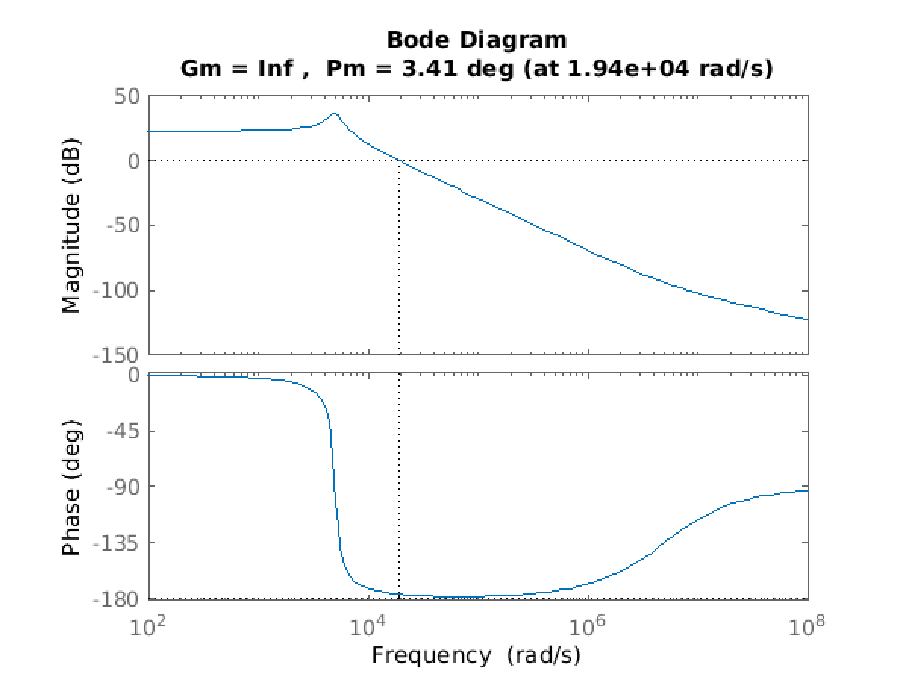
\includegraphics[width=0.45\textwidth]{img/buck.eps}\\
        \textit{\matlab Bode plot of Buck-converter, w/ displayed Phase Margin}
    \end{center}
    
    \begin{matlabcode}
    Vo = 5;
    Vin = 14;
    L = 4e-3;
    C = 10e-6;
    r = 0.02;
    R = 100;
    f_s = 30e3;

    s = tf('s');
    buck = (Vin/(L*C)) * ((1 + s*r*C) / (s^2 + s*(1/(R*C) + r/L) + 1/(L*C)));
    margin(buck)
    \end{matlabcode}

    \section{Controller}
    $$R_i = 10K, K_p=0.1$$\\
    $$R_f = K_p * R_i = 1K$$\\
    $$\mathrm{Phase \; Margin (\; from \; \texttt{margin})}, Pm = 1.9351e4 \; rad/S$$ \\

    Now choosing a $C_f$ value to maintain phase at unity gain, a pole is placed 2 decades before the phase margin computed by \matlab.
    
    $$C_f = \frac{1}{R_f * Pm * 1e-2} = 5.1677uF$$

    $$\therefore \; K_i = \frac{1}{R_i * C_f} = 19.3510$$

    \section{Controller Bode}
    \begin{center}
        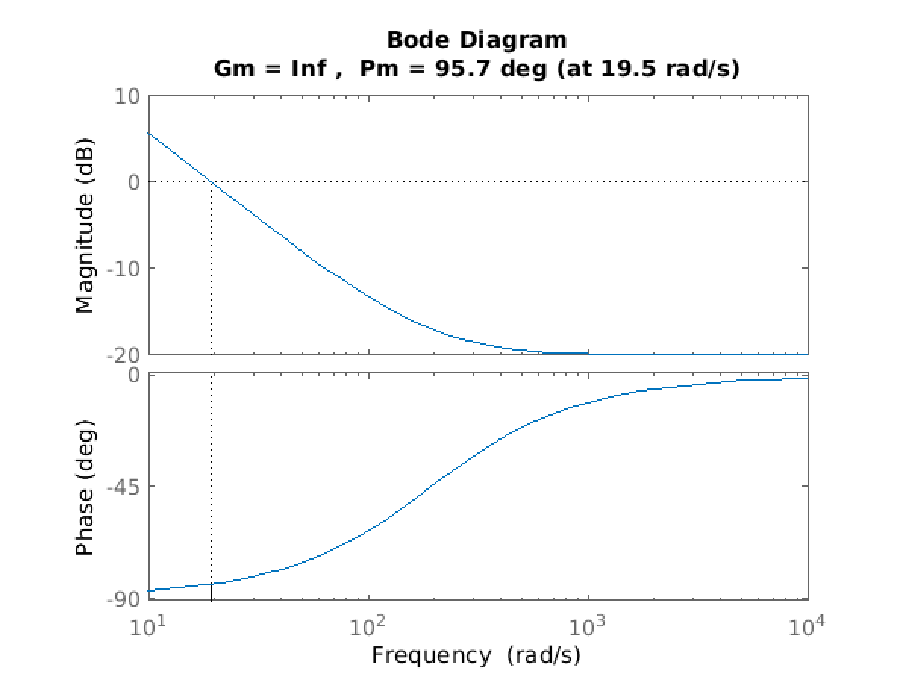
\includegraphics[width=0.45\textwidth]{img/controller.eps}\\
        \textit{Resulting Bode plot of designed controller}
    \end{center}
    
    \begin{matlabcode}
        controller = (Rf + (1/(Cf*s)))/(Ri);
        margin(controller)
    \end{matlabcode}

    \section{Uncontrolled vs Controlled}
    \begin{center}
        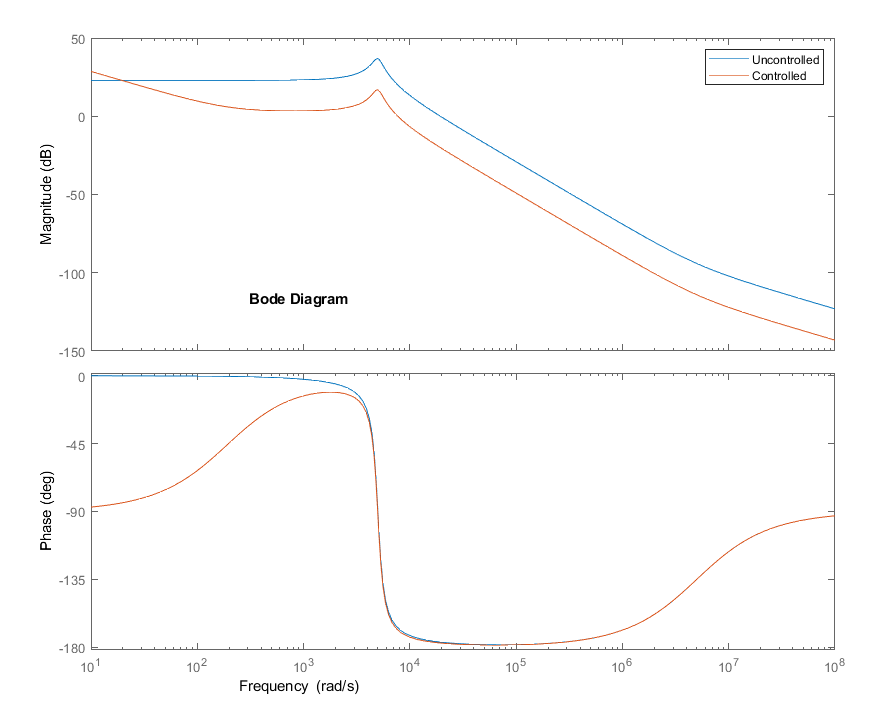
\includegraphics[width=0.45\textwidth]{img/comp.png}\\
        \textit{Comparison between Uncontrolled and Controlled to examine phase behaviour}
    \end{center}
    
    \section{Simulink Model}
    \begin{center}
        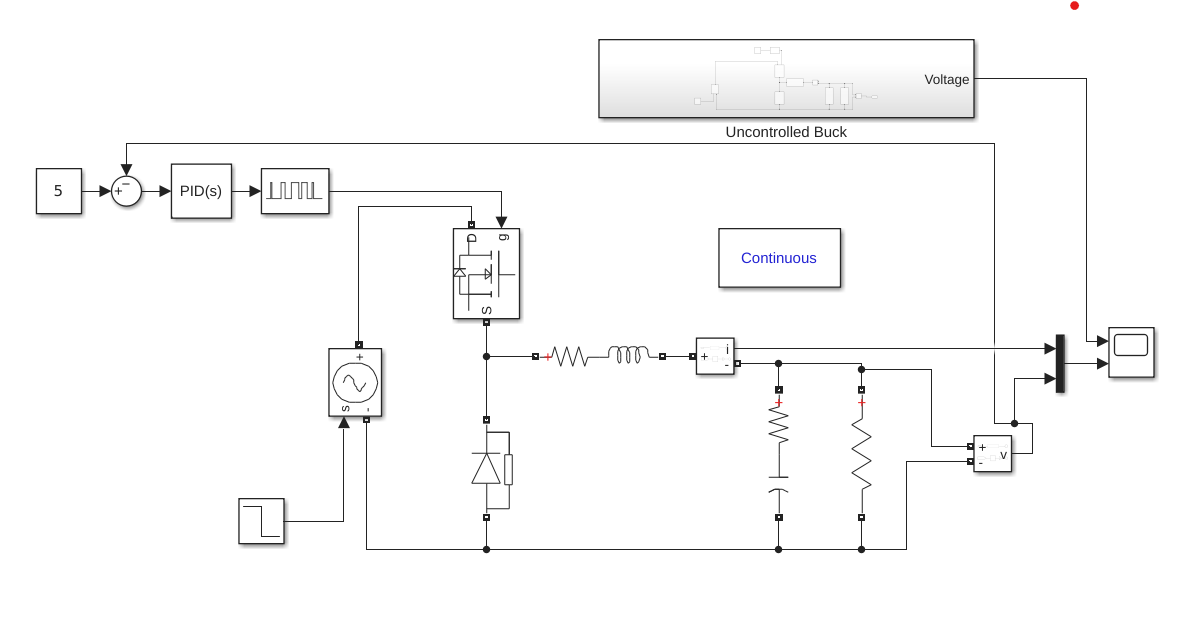
\includegraphics[width=0.75\textwidth]{img/sim.png}\\
        \textit{Simulink Model including controller}

        To implement control in the Simulink model to computed $K_p$ and $K_i$ from the \matlab script at used in a PID block ($K_d = 0$) with output voltage feedback to compute error signal.

        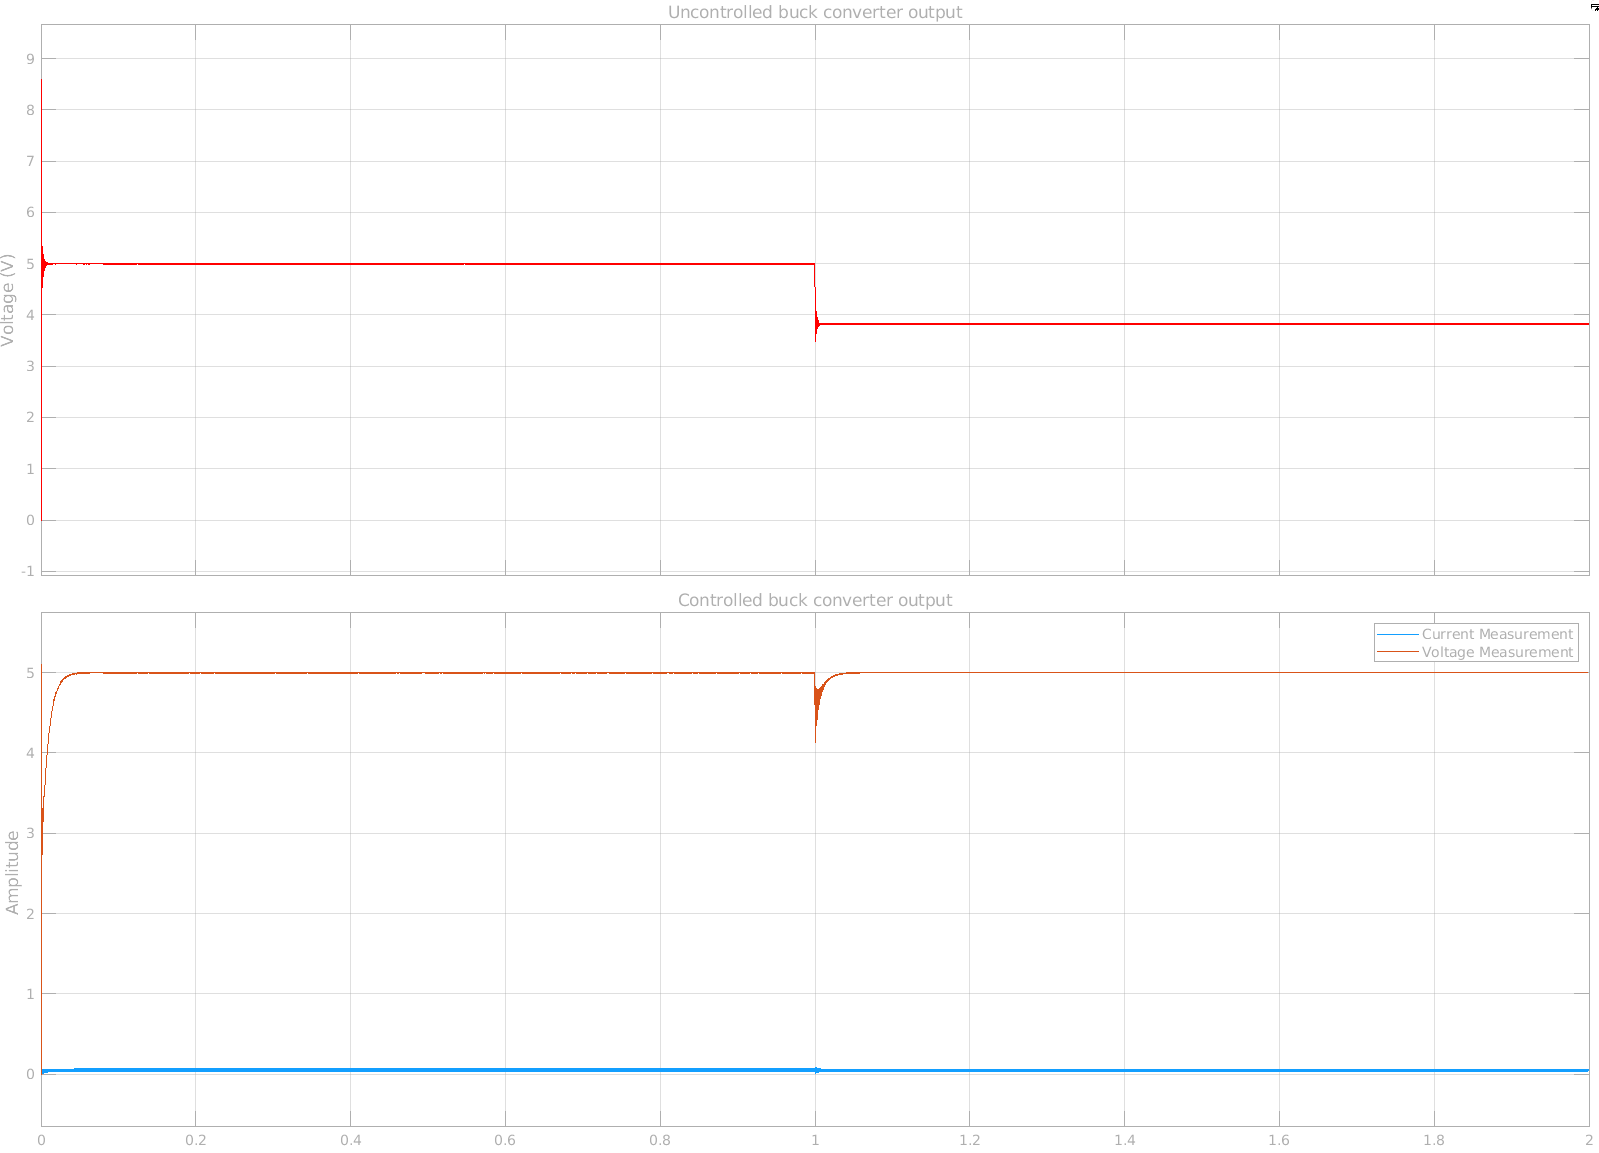
\includegraphics[width=0.45\textwidth]{img/uncontrolled v controlled.png}
        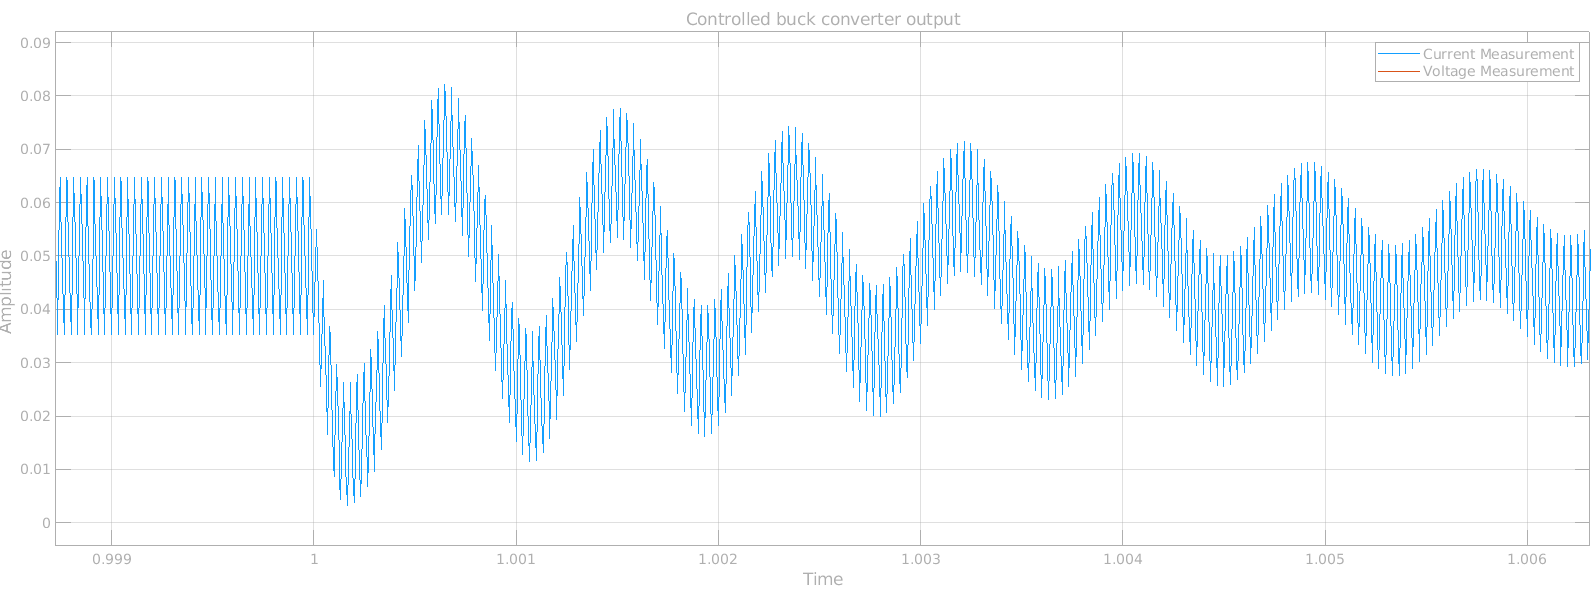
\includegraphics[width=0.45\textwidth]{img/step_zoom.png}\\
        \textit{Left: Controlled vs Uncontrolled Buck converters showing the elimination of steady state error \\  Right: Current ripple at the step of the controlled buck}
    \end{center}
    
    \section{Schematic}
    \begin{center}
        \frame{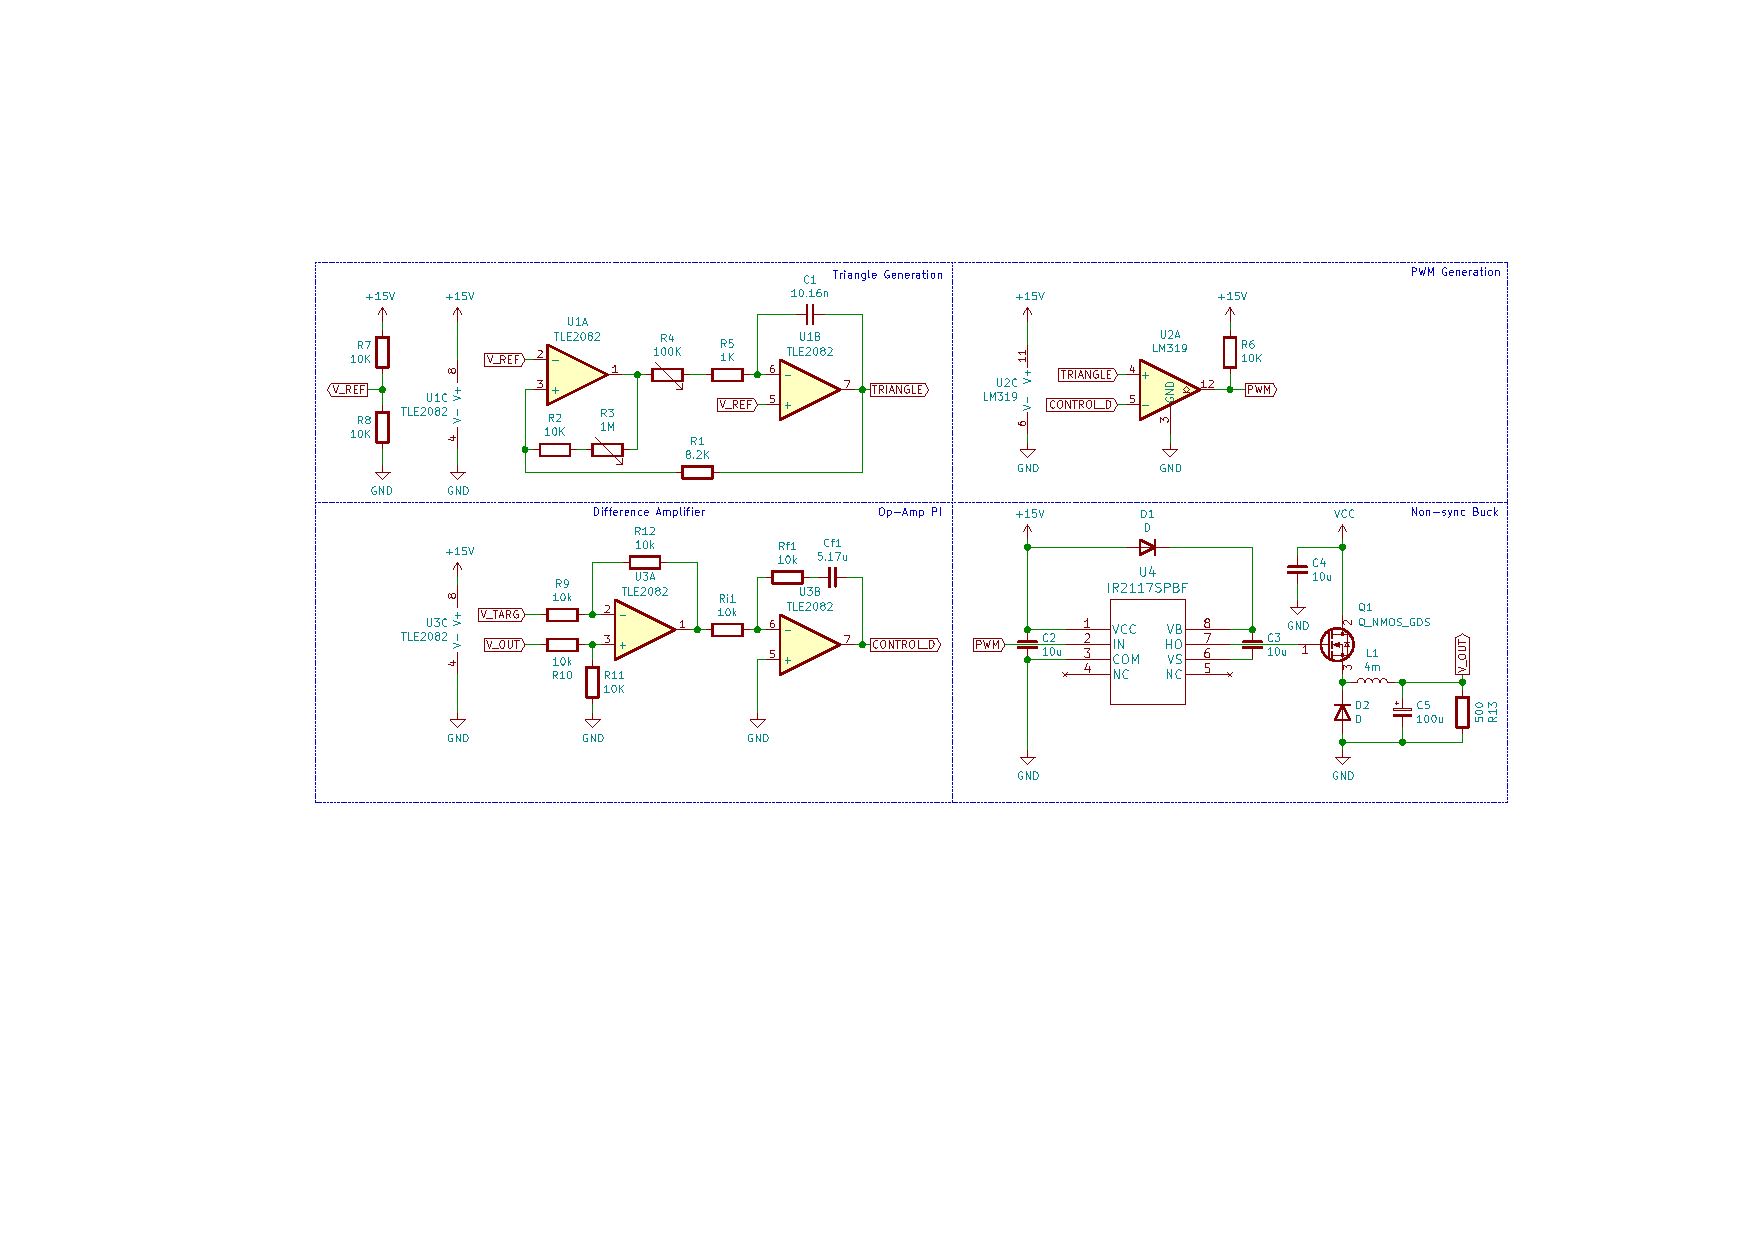
\includegraphics[trim={48mm 70mm 36mm 40mm},clip,width=0.75\textwidth]{img/shem.pdf}}\\
    \end{center}

    \hrule
\end{preview}
\end{document}